\section{Background} \label{sec:background}

In this section, we provide background on the application of deep
learning in robotics, particularly autonomous vehicles.

\subsection{End-to-End Deep Learning for Autonomous Vehicles}

%% - explosion of AI
%% - in particular, application of DNN in perception and control of robotics systems.
%% - end-to-end control is a promising technique.
%%   levine's publications?
%% - examples: nvidia's DAVE-II prototype, forest navigating drone
%% challenge problem: computing at low cost?

To solve the problem of autonomous driving, a standard approach has
been decomposing the problem into multiple sub-problems,
such as lane marking detection, path planning, and low-level
control, which together form a processing pipeline~\cite{Bojarski2016}.
Recently, researchers are exploring another approach that dramatically
simplifies the standard control pipeline by applying deep neural
networks to directly produce control outputs from senor
inputs~\cite{Levine2016}. Figure~\ref{fig:end-to-end-control}
shows the differences between two approaches.

\begin{figure}[h]
  \centering
  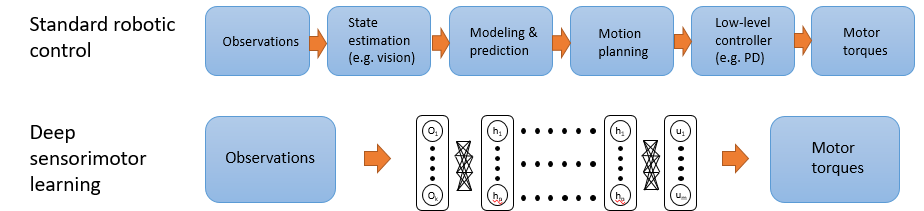
\includegraphics[width=.5\textwidth]{figs/endtoend_redrawn}
  \caption{Standard robotics control vs. DNN based end-to-end
    control. Adopted from ~\cite{Levine2017cs294}.}
  \label{fig:end-to-end-control}
\end{figure}

The use of neural networks for end-to-end control of autonomous
car was first demonstrated in late 1980s~\cite{Pomerleau1989},
using a small 3-layer fully connected neural network; and subsequently
in a DARPA Autonomous Vehicle (DAVE) project in early
2000s~\cite{LeCun:04}, using a 6 layer convolutional neural network
(CNN); and most recently in NVIDIA's DAVE-2
project~\cite{Bojarski2016}, using 9 layer CNN. In all these projects,
the neural network models take raw image pixels as input and directly
produce steering control commands bypassing all intermediary steps and
hand-written rules in conventional robotics control approach. The
NVIDIA's latest effort reports that their trained CNN successfully
self-drive their modified cars in public roads without human
intervention~\cite{Bojarski2016}.

Using deep nueral networks involves two distinct
phases~\cite{NVIDIA2015}. The first
phase is \emph{training} during which the weights of the network is
incrementally updated by backpropating errors it sees from the
training examples. Once the network is trained---i.e., the weights of
the network minimize errors in the training examples---the next phase
is \emph{inferencing} during which unseen data is fed to the network
as input to produce predicted output (e.g., predicted image
classification). In general, the training phase is most compute
intensive and requires high throughput, which is generally not
available on embedded platforms. The inferencing phase, on the
other hand, is relatively less compute intensive and latency becomes
as important, if not more, as compute throughput because many
use-cases have strict real-time requirements (e.g., search query
latency).

%% \cite{Levine2016}: ``In this paper, we aim to answer
%% the following question: does training the perception and control
%% systems jointly end-toend 
%% provide better performance than training each component separately?''

%% \cite{Bojarski2016} nvidia paper
%% ``We trained a convolutional neural network (CNN) to map raw pixels from
%% a sin- gle front-facing camera directly to steering commands.''

%% ``Compared to explicit decomposition of the problem, such as lane
%% marking detec- tion, path planning, and control, our end-to-end system
%% optimizes all processing steps simultaneously. We''

%% UPenn's f1/10 BOM: $3,628.37
%% http://f1tenth.org/
%% http://selfdrivingcars.mit.edu/
%% http://fast.scripts.mit.edu/racecar/
%% https://github.com/mit-racecar
%% https://mit-racecar.github.io/

\subsection{Embedded Computing Platforms for Real-Time Inferencing}
Real-time embedded systems, such as an autonomous vehicle, present
unique challenges for deep learning as the computing platforms of such
systems must satisfy two often conflicting goals~\cite{Otterness2017}:
%% Recent successes in AI, including NVIDIA's DAVE-2 showing, are due
%% in large part to the increased computing performance,
%% which afforded researchers to train and use ever deeper neural networks with
%% high accuracy.
%% For practical applications, the computer platform in an
%% autonomous vehicle must satisfy two often conflicting goals:
On the one hand, the platform must provide 
enough computing capacity for real-time processing of computationally
expensive AI workloads (deep neural networks);
On the other hand, the platform must also satisfy various
constrains such as cost, size, weight, and power consumption limits.

Accelerating AI workloads, especially inferencing
operations, has gotten a lot of attentions from academia and industry
in recent years as applications of deep learning are broadening to
areas real-time embedded systems such as autonomous vehicles. These
efforts include development of various heterogeneous architecture
based system-on-a-chips (SOCs) that may include multiple cores, GPU,
DSP, FPGA and neural network optimized ASIC hardware~\cite{Jouppi2017}.
Consolidating multiple tasks on SoCs with lots of shared hardware
resources while guaranteeing real-time performance is also an active
research area, which is orthogonal to improving raw
performance. Consolidation is necessary for efficiency but unmanaged 
interference can nullify the benefits of consolidation~\cite{Kim2016}.
Because of these reasons, finding a right computing platform is
non-trivial task, one that requires deep understanding of the
workloads and the hardware platform that executes the workloads.

The primary objectives of this study are (1) to understand the
necessary computing performance for applying AI technology based
robotics systems, and (2) what kind of computing architecture and
runtime supports are most appropriate for such workload. Toward to
achieve these goals, we implement a low-cost autonomous car platform
as a case-study and systematically conduct experiments, as we will 
describe in the subsequent sections.
